\documentclass[journal,12pt,twocolumn]{IEEEtran}

\usepackage{setspace}
\usepackage{gensymb}

\singlespacing


\usepackage[cmex10]{amsmath}

\usepackage{amsthm}

\usepackage{mathrsfs}
\usepackage{txfonts}
\usepackage{stfloats}
\usepackage{bm}
\usepackage{cite}
\usepackage{cases}
\usepackage{subfig}

\usepackage{longtable}
\usepackage{multirow}

\usepackage{enumitem}
\usepackage{mathtools}
\usepackage{steinmetz}
\usepackage{tikz}
\usepackage{circuitikz}
\usepackage{verbatim}
\usepackage{tfrupee}
\usepackage[breaklinks=true]{hyperref}
\usepackage{graphicx}
\usepackage{tkz-euclide}
\usepackage{float}

\usetikzlibrary{calc,math}
\usepackage{listings}
    \usepackage{color}                                            %%
    \usepackage{array}                                            %%
    \usepackage{longtable}                                        %%
    \usepackage{calc}                                             %%
    \usepackage{multirow}                                         %%
    \usepackage{hhline}                                           %%
    \usepackage{ifthen}                                           %%
    \usepackage{lscape}     
\usepackage{multicol}
\usepackage{chngcntr}

\DeclareMathOperator*{\Res}{Res}

\renewcommand\thesection{\arabic{section}}
\renewcommand\thesubsection{\thesection.\arabic{subsection}}
\renewcommand\thesubsubsection{\thesubsection.\arabic{subsubsection}}

\renewcommand\thesectiondis{\arabic{section}}
\renewcommand\thesubsectiondis{\thesectiondis.\arabic{subsection}}
\renewcommand\thesubsubsectiondis{\thesubsectiondis.\arabic{subsubsection}}


\hyphenation{op-tical net-works semi-conduc-tor}
\def\inputGnumericTable{}                                 %%

\lstset{
%language=C,
frame=single, 
breaklines=true,
columns=fullflexible
}
\begin{document}


\newtheorem{theorem}{Theorem}[section]
\newtheorem{problem}{Problem}
\newtheorem{proposition}{Proposition}[section]
\newtheorem{lemma}{Lemma}[section]
\newtheorem{corollary}[theorem]{Corollary}
\newtheorem{example}{Example}[section]
\newtheorem{definition}[problem]{Definition}

\newcommand{\BEQA}{\begin{eqnarray}}
\newcommand{\EEQA}{\end{eqnarray}}
\newcommand{\define}{\stackrel{\triangle}{=}}
\bibliographystyle{IEEEtran}
\providecommand{\mbf}{\mathbf}
\providecommand{\pr}[1]{\ensuremath{\Pr\left(#1\right)}}
\providecommand{\qfunc}[1]{\ensuremath{Q\left(#1\right)}}
\providecommand{\sbrak}[1]{\ensuremath{{}\left[#1\right]}}
\providecommand{\lsbrak}[1]{\ensuremath{{}\left[#1\right.}}
\providecommand{\rsbrak}[1]{\ensuremath{{}\left.#1\right]}}
\providecommand{\brak}[1]{\ensuremath{\left(#1\right)}}
\providecommand{\lbrak}[1]{\ensuremath{\left(#1\right.}}
\providecommand{\rbrak}[1]{\ensuremath{\left.#1\right)}}
\providecommand{\cbrak}[1]{\ensuremath{\left\{#1\right\}}}
\providecommand{\lcbrak}[1]{\ensuremath{\left\{#1\right.}}
\providecommand{\rcbrak}[1]{\ensuremath{\left.#1\right\}}}
\theoremstyle{remark}
\newtheorem{rem}{Remark}
\newcommand{\sgn}{\mathop{\mathrm{sgn}}}
\providecommand{\abs}[1]{\lvert#1\vert}
\providecommand{\res}[1]{\Res\displaylimits_{#1}} 
\providecommand{\norm}[1]{\lVert#1\rVert}
%\providecommand{\norm}[1]{\lVert#1\rVert}
\providecommand{\mtx}[1]{\mathbf{#1}}
\providecommand{\mean}[1]{E[ #1 ]}
\providecommand{\fourier}{\overset{\mathcal{F}}{ \rightleftharpoons}}
%\providecommand{\hilbert}{\overset{\mathcal{H}}{ \rightleftharpoons}}
\providecommand{\system}{\overset{\mathcal{H}}{ \longleftrightarrow}}
	%\newcommand{\solution}[2]{\textbf{Solution:}{#1}}
\newcommand{\solution}{\noindent \textbf{Solution: }}
\newcommand{\cosec}{\,\text{cosec}\,}
\providecommand{\dec}[2]{\ensuremath{\overset{#1}{\underset{#2}{\gtrless}}}}
\newcommand{\myvec}[1]{\ensuremath{\begin{pmatrix}#1\end{pmatrix}}}
\newcommand{\mydet}[1]{\ensuremath{\begin{vmatrix}#1\end{vmatrix}}}
\numberwithin{equation}{subsection}
\makeatletter
\@addtoreset{figure}{problem}
\makeatother
\let\StandardTheFigure\thefigure
\let\vec\mathbf
\renewcommand{\thefigure}{\theproblem}
\def\putbox#1#2#3{\makebox[0in][l]{\makebox[#1][l]{}\raisebox{\baselineskip}[0in][0in]{\raisebox{#2}[0in][0in]{#3}}}}
     \def\rightbox#1{\makebox[0in][r]{#1}}
     \def\centbox#1{\makebox[0in]{#1}}
     \def\topbox#1{\raisebox{-\baselineskip}[0in][0in]{#1}}
     \def\midbox#1{\raisebox{-0.5\baselineskip}[0in][0in]{#1}}
\vspace{3cm}
\title{ASSIGNMENT 6}
\author{A.keerthana}
\maketitle
\newpage
\bigskip
\renewcommand{\thefigure}{\theenumi}
\renewcommand{\thetable}{\theenumi}
Download all python codes from 
\begin{lstlisting}
https://github.com/Atlakeerthana/Assignment6/tree/main/Assignment6
\end{lstlisting}
%
and latex-tikz codes from 
%
\begin{lstlisting}
https://github.com/Atlakeerthana/Assignment6/tree/main/Assignment6
\end{lstlisting}
%
\section{Question No 2.74(e)}
In each of the following find the equation for the ellipse that satisfies the given conditions:
\begin{enumerate}[label=\alph*.]
\item Conjugate axis length= 24,
foci= \myvec{0\\\pm13}
\end{enumerate}
%
\section{Solution}
Given that,
\begin{align}
\text{Conjugate axis length }&= 2b = 24 
\\
\therefore \text{Length of semi major axis, } b&=12\label{eqA}
  \\
\text{Foci}&=\vec{F} = \myvec{0\\\pm13} \label{eqB}
\end{align}
\begin{lemma}
\label{lemma}
The standard equation of an ellipse is given by:
\begin{align}
\frac{\vec{y}^{\top}D\vec{y}}{\vec{u}^{\top}\vec{V}^{-1}\vec{u}-f}&=1
\\
\text{where, } D &=\myvec{\lambda_1& 0 \\ 0 & \lambda_2}
\end{align}
\end{lemma}
\begin{lemma}
The coordinates of foci $\vec{F}$ of ellipse  with y-axis as major axis are:
 \begin{align}
  \vec{F} &= \myvec{0\\ \pm \brak{\sqrt{\frac{(\vec{u}^T\vec{V}^{-1}\vec{u}-f)(\lambda_2-\lambda_1)}{\lambda_1\lambda_2}}}} \label{eqC}
\end{align}
Also,the length of semi major axis, a is
\begin{align}
  a = \sqrt{\frac{\vec{u}^{\top}\vec{V}^{-1}\vec{u}-f}{\lambda_1}} 
  \end{align}
and the length of semi minor axis, b is
  \begin{align}
  b &= \sqrt{\frac{\vec{u}^{\top}\vec{V}^{-1}\vec{u}-f}{\lambda_2}} \label{eqD}
 \end{align}
\end{lemma}
\begin{enumerate}
\item From \eqref{eqD} length of semi-minor axis is:
\begin{align}
 \sqrt{\frac{\vec{u}^{\top}\vec{V}^{-1}\vec{u}-f}{\lambda_2}} &= b
\\
 \frac{\vec{u}^{\top}\vec{V}^{-1}\vec{u}-f}{\lambda_2} &= b^2
\\
\implies \lambda_2&=\frac{\vec{u}^{\top}\vec{V}^{-1}\vec{u}-f}{b^2}\label{eqF} 
\end{align}
\item From \eqref{eqC}, the focus of ellipse is given as:
\begin{align}
 \vec{F} &= \myvec{0\\\pm \brak{\sqrt{\frac{(\vec{u}^T\vec{V}^{-1}\vec{u}-f)(\lambda_2-\lambda_1)}{\lambda_1\lambda_2}}}}
 \end{align}
 or
 \begin{align}
\norm{\vec{F}}^2 &= \frac{(\vec{u}^T\vec{V}^{-1}\vec{u}-f)(\lambda_2-\lambda_1)}{\lambda_1\lambda_2}
 \\
\norm{\vec{F}}^2 &= \frac{\vec{u}^{\top}\vec{V}^{-1}\vec{u}-f}{\lambda_1}-\frac{\vec{u}^{\top}\vec{V}^{-1}\vec{u}-f}{\lambda_2} \label{eqE}
 \end{align}
\item Putting value of $\lambda_2$ from \eqref{eqF} in above equation, we get:
\begin{align}
    \norm{\vec{F}}^2&= \frac{\vec{u}^{\top}\vec{V}^{-1}\vec{u}-f}{\lambda_1}-b^2
    \\
    \norm{\vec{F}}^2+b^2 &= \frac{\vec{u}^{\top}\vec{V}^{-1}\vec{u}-f}{\lambda_1}
    \\
 \implies \lambda_1 &= \frac{\vec{u}^{\top}\vec{V}^{-1}\vec{u}-f}{\norm{\vec{F}}^2+b^2}\label{eq1}
    \end{align}
    \item \textit{For finding $\lambda_2$}:
\begin{itemize}
    \item From \eqref{eqF} we have:
\begin{align}
\lambda_2&=\frac{\vec{u}^{\top}\vec{V}^{-1}\vec{u}-f}{b^2}
\\
\implies \lambda_2&=\frac{\vec{u}^{\top}\vec{V}^{-1}\vec{u}-f}{144} \brak{\because b=12} \label{eqH}
\end{align}
\end{itemize}
\item \textit{For finding $\lambda_1$:}
\begin{itemize}
\item Putting value of b from \eqref{eqA} and $\vec{F}$ from \eqref{eqB} in equation \eqref{eq1},we get:
\begin{align}
   \lambda_1&= \frac{\vec{u}^{\top}\vec{V}^{-1}\vec{u}-f}{\brak{\sqrt{0^2+13^2}}^2+12^2}\\
     \lambda_1&= \frac{\vec{u}^{\top}\vec{V}^{-1}\vec{u}-f}{169+144}\\
      \lambda_1&= \frac{\vec{u}^{\top}\vec{V}^{-1}\vec{u}-f}{313}\label{eqG}
\end{align}
\end{itemize}
\item Using lemma \eqref{lemma},the standard equation of ellipse is given by :
\begin{align}
\frac{\vec{y}^{\top}D\vec{y}}{\vec{u}^{\top}\vec{V}^{-1}\vec{u}-f}=1
\end{align}
\begin{align}
\implies \frac{\vec{y}^{\top}\myvec{\lambda_1& 0 \\ 0 & \lambda_2}\vec{y} }{\vec{u}^{\top}\vec{V}^{-1}\vec{u}-f}=1
\end{align}
\item Putting \eqref{eqH} and \eqref{eqG} in above equation we get:
\begin{align}
\implies \vec{y}^{\top}\myvec{\frac{1}{313}& 0 \\ 0 & \frac{1}{144}}\vec{y}=1
\end{align}
which is the required equation of ellipse.
\item The Plot of ellipse is:
\numberwithin{figure}{section}
\begin{figure}[!ht]
    \centering
    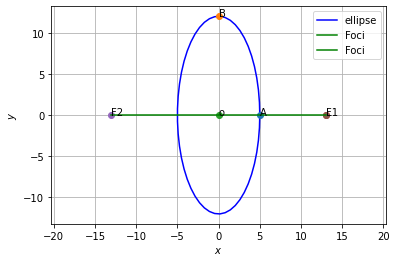
\includegraphics[width=\columnwidth]{figure6.png}
    \caption{Ellipse $\frac{x^2}{313} + \frac{y^2}{144} = 1$}
    \label{fig:ellipse}
\end{figure} 
\end{enumerate}
\end{document}